\documentclass{beamer}
\usepackage[hungarian]{babel}
\usepackage[utf8]{inputenc}
\usepackage{amsmath}
\usepackage{graphicx}
\graphicspath{{./images/}}
\usepackage[
    backend=bibtex,
    style=numeric,
    citestyle=numeric,
    sorting=none]
    {biblatex}
\addbibresource{citations}
\usetheme{Boadilla}

\title{Nyilvános kulcsú titkosítás}
\author{Bolyki Balázs}
\institute{Miskolci Egyetem}
\date{\today}

\begin{document}

\titlepage

\begin{frame}
    \frametitle{Szimmetrikus titkosítás}

    \textbf{Pár szó a szimmetrikus titkosításról...}

    \begin{itemize}
        \item A szimmetrikus titkosításnál egyetlen kulcs van.
        \item A kulcs segítségével lehet titkosítani az üzenetet és megfejteni a titkosított szöveget.
        \item Az üzenet addig lesz titkos, míg az illetéktelen nem ismerik a kulcsot.
        \item Probléma: hogyan osszák meg egymással a kulcsát?
        \item Megoldási lehetőség: nyilvános kulcsú titkosítás.
    \end{itemize}
\end{frame}

\begin{frame}
    \frametitle{Alapgondolat}
    \textbf{Kérdés}: Hogyan tud két fél titkosítva információt cserélni egymással úgy, hogy soha nem találkoztak?

    \textbf{Válasz}: Nyilvános kulcsú (vagy aszimmetrikus) titkosítással.

    \textbf{Két kulcs van}: Egy publikus és egy privát.

    \textbf{Postás példa}:

    \begin{itemize}
        \item Laci szeretne elküldeni egy dobozt Karcsinak.
        \item A dobozt csak Karcsi tudhatja kinyitni.
        \item Ezért Karcsi a postán hagy egy lakatot, amihez rendelkezik kulccsal.
        \item Laci a postára megy, felrakja a dobozra Karcsi lakatját, és elküldi postán a dobozt.
        \item Karcsi a kulcsával leszedi a lakatot, és kinyitja a dobozt.
    \end{itemize}

    A példában a lakat a nyilvános kulcs, a lakatkulcs pedig a privát kulcs.

\end{frame}

\begin{frame}
    \frametitle{Működés szabadnyelvi leírása}

    \textbf{Kulcsok}:
    \begin{itemize}
        \item \textbf{Publikus kulcs}: Mindenki számára elérhető.
        \item \textbf{Privát kulcs}: Csak az adott fél számára elérhető.
    \end{itemize}
    \textbf{Megkötés}: A publikus kulccsal titkosított üzenet csak a privát kulccsal dekódolható.

    \textbf{Megfordítható (\textit{reversible}) abban az esetben, ha } a privát kulccsal titkosított
    üzenet dekódolható a publikus kulccsal.

    \textbf{Hol használják}:
    \begin{itemize}
        \item TLS/SSL (certificate authority)
        \item Digitális aláírás
        \item Blockchain (kriptovaluta)
    \end{itemize}
\end{frame}

\begin{frame}
    \frametitle{Formális meghatározás}

    Legyen $\{E_e: e \in K\}$ titkosítási (\textit{encryption}) transzformációk halmaza, míg $\{D_d: d \in K\}$
    pedig visszafejtési transzformációk halmaza, ahol $K$ a kulcstér.

    Vegyünk egy párt ezek közül: $(E_e, D_d)$. Ekkor:

    \begin{itemize}
        \item $E_e(m) = c$, ahol $m$ (\textit{message}) egy üzenetszó, $c$ pedig egy titkosított szöveg.
        \item $D_d(c) = m$, tehát a $D_d$ transzformációkkal visszafejthető az $E_e$ által előállított $c$ titkosított
              szövegből $m$ üzenetszó.
    \end{itemize}

    \textbf{A következőknek teljesülnie kell:}

    \begin{itemize}
        \item $E_e$ ismeretében és $D_d$ ismeretének hiányában $c$ kódszóból nem kivitelezhető $m$ előállítása (belátható
              időn belül).
        \item Ebből az is következik, hogy $E_e$ ismeretében $D_d$ kikövetkeztetése szintén kivitelezhetetlen.
    \end{itemize}

    \textbf{Még ha egy támadó el is fogja a $B$-nek szóló üzeneteket, akkor sem fogja tudni elolvasni őket.}
\end{frame}

\begin{frame}
    \frametitle{Szemléltetés}

    \begin{figure}[h]
        \centering
        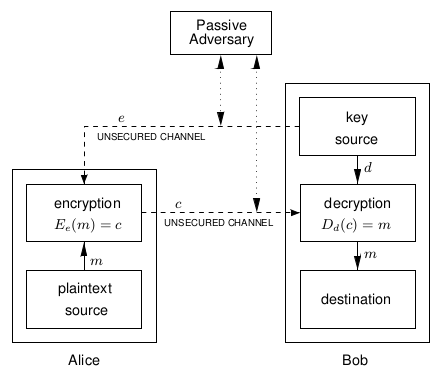
\includegraphics[scale=0.5]{encryption.png}
        \caption{Publikus kulcsú titkosítás \cite{Menezes2001}}
        \label{fig_encryption}
    \end{figure}
\end{frame}

\begin{frame}
    \frametitle{Autentikációs probléma}

    A publikus kulcsú titkosításnál is felvetődik a \textit{man-in-the-middle} probléma.

    \begin{itemize}
        \item Tegyük fel, hogy $A$ üzenetet akar küldeni $B$-nek.
        \item Ahhoz, hogy ezt a publikus kulcsú titkosítás alkalmazásával megtehesse, először meg kell szereznie a
              publikus kulcsot.
        \item A publikus kulcs megszerzése nem biztonságos csatornán keresztül történik (ha biztonságos lenne a csatorna,
              akkor akár szimmetrikus kulcsú titkosítást is használhatnánk).
        \item Tegyük fel, hogy $A$ üzenetet küld, amiben elkéri $B$ publikus kulcsát, viszont $C$ elfogja ezt az üzenetet,
              és elküldi $A$-nak a saját publikus kulcsát.
        \item Ebben az esetben a $B$-nek küldött üzeneteket már $C$ nem csak elfogja, hanem el is tudja olvasni.
    \end{itemize}

    \textbf{Következtetés:} Meg kell bizonyosodni róla, hogy a publikus kulcs, amit $A$ megkap valóban $B$-hez tartozik.
\end{frame}

\begin{frame}
    \frametitle{Digitális aláírás}

    Digitális aláírással hitelesíthetjük a kapott kulcsot. Ez akkor kivitelezhető, ha a titkosítás megfordítható, azaz

    \[D_d(E_e(m)) = E_e(D_d(m)) = m, \forall m \in M \text{ ahol $M$ az üzenettér}\]

    Szintén szükséges, hogy az üzenettér és a kódszó tér ugyanaz legyen: $M = C$, ahol $C$ a kódszó tér.

    Tehát felhasználhatjuk $D_d$ transzformációkat arra, hogy létrehozzunk egy kódszót, amelyet $E_e$ transzformációkkal
    lehet visszaalakítani üzenetszóvá.
\end{frame}

\begin{frame}
    \frametitle{Digitális aláírás 2}

    Legyen adott az üzenetszó térnek egy altere ($M'$), aminek mérete lényegesen kisebb, mint $M$ mérete, és az elemei
    felismerhetőek valamilyen tulajdonságuk alapján.

    $M'$ elemeinek különleges tulajdonsága publikus.

    A digitális aláírás elkészítéséhez használt függvény $D_d$.

    A digitális aláírás verifikációjához használt függvény $V_A$, amely igazat ad, ha hiteles az üzenet, hamisat, ha
    nem.

    Jelölje $s$ a digitális aláírást, ami ebben az esetben $D_d(m) = s$, ahol $m \in M$.

    \begin{equation}
        V_A =
        \begin{cases}
            true  & \text{ha $E_e(s) \in M'$,} \\
            false & \text{egyébként.}
        \end{cases}
    \end{equation}

\end{frame}

\begin{frame}
    \frametitle{Digitális aláírás 3}

    \textbf{További magyarázat:}

    \begin{itemize}
        \item A publikus kulcs fogadója a digitális szignatúrát megkísérli hitelesíteni.
        \item Ezt úgy teszi, hogy $E_e$ transzformációkat elvégzi $s$ szignatúrán.
        \item Ha a transzformációk eredménye egy olyan $m$, amire az ismert különleges tulajdonság igaz, akkor hiteles a kulcs.
    \end{itemize}

    Fontos az, hogy $M'$ mérete sokkal kisebb, mint $M$ mérete, így ugyanis az "egzisztenciális hamisítás" nagyon kis eséllyel
    lesz sikeres.

    Egzisztenciális hamisításról akkor beszélünk, ha a hamisító vesz egy véletlenszerű $s$ szignatúrát, és keres hozzá egy
    $m \in M$ üzenetet, amit az hitelesíteni tud. Így meghamisíthatja a hitelesítést is.

    Ha csak $m \in M'$ üzenetet fogadunk el hitelesnek, akkor ez a fajta hamisítás sokkal kisebb valószínűséggel kivitelezhető.
\end{frame}

\begin{frame}
    \frametitle{Szimmetrikus vs. aszimmetrikus titkosítás 1.}

    \textbf{Szimmetrikus titkosítás előnyei:}
    \begin{itemize}
        \item Nagy mennyiségű adatot lehet vele gyorsan titkosítani.
        \item A kulcsok relatívan rövidek.
        \item Több különböző algoritmus (akár több különböző kulccsal) láncolható, hogy belőlük még erősebb titkosítás
              jöjjön létre.
        \item Messzebbre nyúlik a története, mint a nyilvános kulcsú titkosításnak.
    \end{itemize}

    \textbf{Szimmetrikus titkosítás hátrányai:}
    \begin{itemize}
        \item A kulcs titkosságára mindkét oldalon ügyelni kell (küldő és fogadó oldalon is).
        \item Nagy hálózatok esetén nehéz számontartani a sok kulcsot a küldő-fogadó párokhoz.
        \item A kulcsoknak feltehetőleg gyakran kell változnia két fél között (akár minden kommunikációs \textit{session}
              esetén különbözőnek kell lennie).
    \end{itemize}
\end{frame}

\begin{frame}
    \frametitle{Szimmetrikus vs. aszimmetrikus titkosítás 2.}

    \textbf{Aszimmerikus titkosítás előnyei:}
    \begin{itemize}
        \item Csak a privát kulcsot kell titokban tartani.
        \item Egy publikus-privát kulcspár sokáig változatlan maradhat.
        \item Könnyebb vele a digitális aláírás megvalósítása.
    \end{itemize}

    \textbf{Aszimmetrikus titkosítás hátrányai:}
    \begin{itemize}
        \item Lényegesen lassabb, mint a szimmetrikus titkosítás.
        \item Lényegesen nagyobbak a kulcsok, mint a szimmetrikus kulcsok.
        \item A biztonságosságuk nem bizonyított; arra alapoznak, hogy a bennük felmerülő számelméleti nehézségeket tovább
              tart megoldani, mint ameddig a kulcspárok használatban lesznek.
        \item Fiatalabb terület, mint a szimmetrikus titkosítás, ugyanis a 70-es évek közepétől kezdve használják.
    \end{itemize}
\end{frame}

\begin{frame}
    \frametitle{RSA}

    \begin{itemize}
        \item A legismertebb publikus kulcsú titkosítás az RSA algoritmus.
        \item Az algoritmus a kidolgozóiról kapta a nevét: Ron \textbf{R}ivest, Adi \textbf{S}hamir és \textbf{L}eonard Adleman.
        \item 1977-ben publikálták.
        \item Egy ekvivalens verzióját 1973-ban már Clifford Cock már kidolgozta a GCHQ (Government Communication Headquarters),
              amelyet csak 1997-ben hoztak nyilvánosságra.
    \end{itemize}
\end{frame}

\begin{frame}
    \frametitle{ECDSA: Elliptic Curve Digital Signature Algorithm \cite{ecdsa}}

    \begin{itemize}
        \item Széles körben használt digitális aláírás algoritmus.
        \item \textit{Bitcoin security} alapja.
        \item TLS is ezt az algoritmust használja.
        \item Rövidebb kulcsot használ, mint az RSA algoritmus.
    \end{itemize}
\end{frame}

\begin{frame}
    \frametitle{Felhasznált irodalom}

    \printbibliography[heading=bibintoc]
\end{frame}

\begin{frame}
    \Huge
    \textbf{Köszönöm a figyelmet!}
\end{frame}

\end{document}